\chapter{连续反应器与工业过程}\label{ch:b2:continuous-reactors}

在实验室里，反应在烧瓶中进行：加入试剂，
混合物搅拌一小时，终止反应，
分离出生成物。以吨计生产同一产品的工厂，
做法则不同。其反应器从不排空：反应物
从一端持续流入，生成物从另一端流出，日夜不停，
内部组成不随时间改变。于是，“多长时间？”
便被两个问题取代：给定转化率时反应器应多大，
以及如何在反应热使反应器温度失控之前将其移走？
本章针对两种理想连续反应器，
即搅拌釜与管式反应器，写出物料与能量衡算，
比较二者，并说明反应器可能存在多种稳态，
其中之一为热失控。

\begin{recall}
本科一年级分册内容：反应速率、速率方程与反应级数，
封闭反应器（现称间歇反应器）的积分速率方程，半衰期，
阿伦尼乌斯定律 $k = A\,\mathrm e^{-E_a/RT}$，连串反应。
\Cref{ch:b2:reaction-enthalpy}：恒压下放出的热量；
\cref{ch:b2:equilibrium-shifts}：单程转化率、循环。
来自物理学：稳定流动中开口系统的衡算（流入量减去
流出量等于累积量）。
\end{recall}

\begin{omfigure}
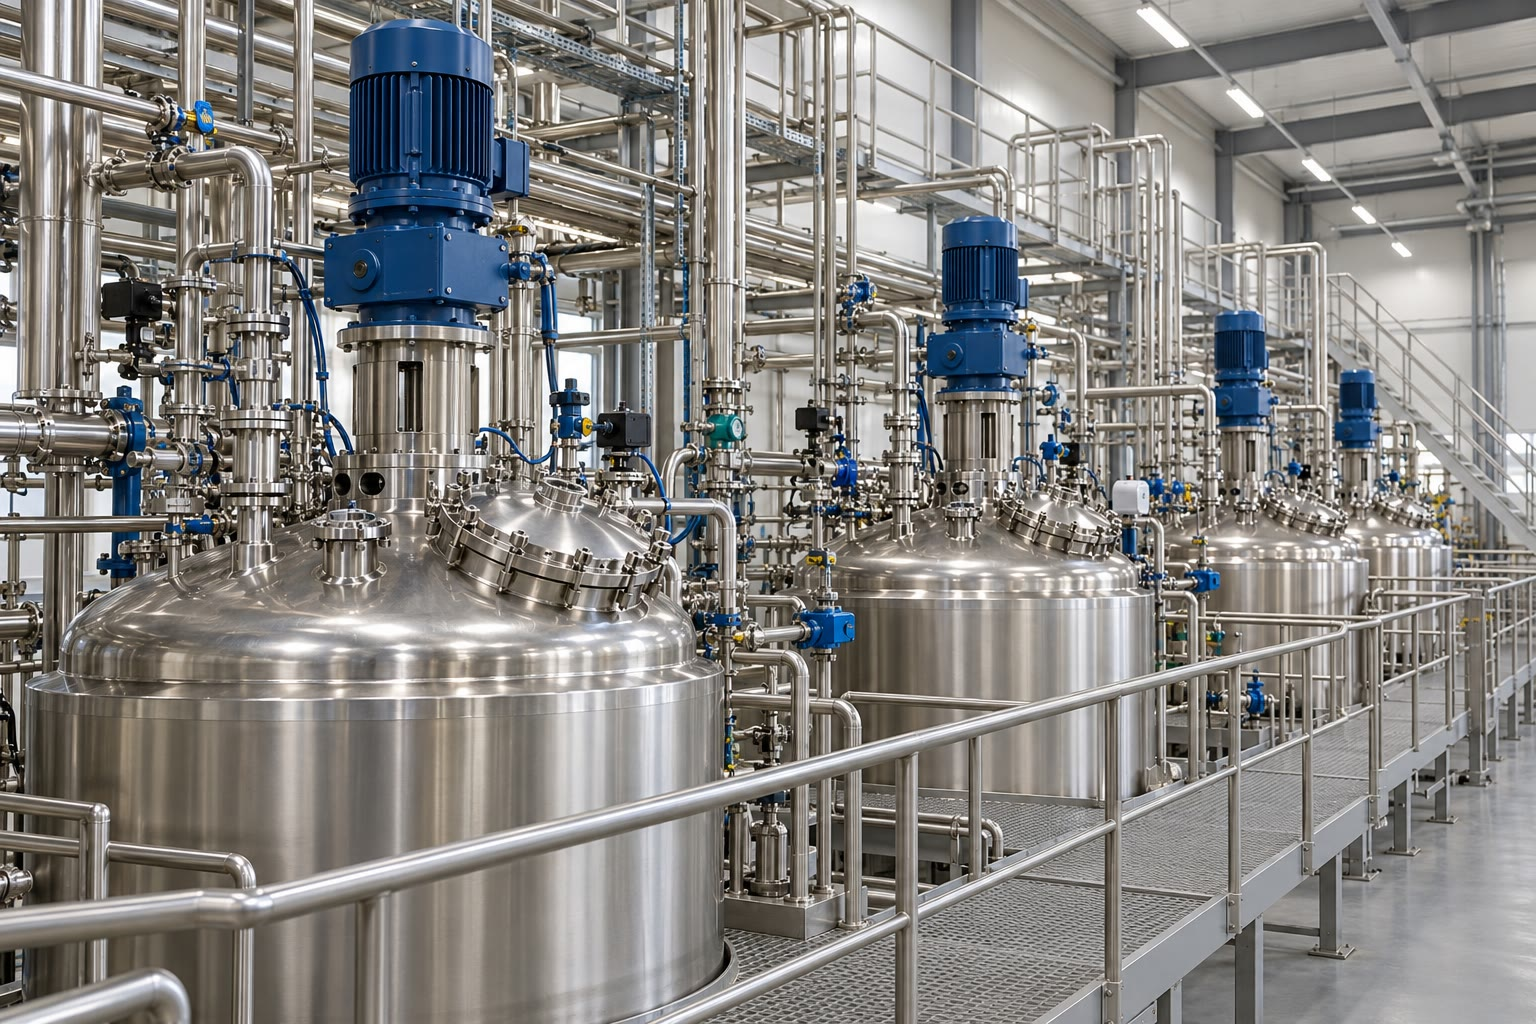
\includegraphics[width=0.6\linewidth]{images/book3/ai/b2-05-stirred-tanks.jpg}

{\small 化工厂中的搅拌釜式反应器：每个釜都配有
电动机与齿轮箱，搅拌轴伸入反应混合物中；
管道输送进料，并引出生成物与冷却水。}
\end{omfigure}

\section{从间歇到连续}

\begin{definition}[反应器类型]\label{def:b2:continuous-reactors:reactors}
称\emph{间歇反应器}\index{间歇反应器}为封闭容器，其中
反应在无物质流入或流出的情况下进行。
\emph{连续反应器}\index{连续反应器}则是
有稳定物流穿过的反应器。两种理想连续反应器可作为模型：
\begin{itemize}
  \item \emph{连续搅拌釜式反应器}\index{连续搅拌釜式反应器}
（CSTR），搅拌充分，使其中的内容物
        组成处处均匀，因而与流出的物流相同；
  \item \emph{平推流反应器}\index{平推流反应器}（PFR），一根管道
        流体流过管道，沿流动方向不混合，各段流体
        像活塞一样推进并同时发生反应。
\end{itemize}
\end{definition}

连续反应器内部的任何量都不随时间变化时，
称其处于\emph{稳态运行}。各处的流量、温度与组成
均保持恒定。考虑单一反应
$\mathrm A \to$ 生成物，液体进料，密度恒定（故进出口的
体积流量 $Q_v$ 相同），入口处
浓度为 $c_{A,0}$。

\begin{definition}[停留时间]\label{def:b2:continuous-reactors:residence-time}
连续反应器的\emph{停留时间}\index{停留时间}，
指体积为 $V$、以体积流量 $Q_v$ 进料的反应器，
其值为 $\tau = V/Q_v$，即一段流体在其中平均停留的时间。
\end{definition}

\begin{definition}[转化率]\label{def:b2:continuous-reactors:conversion}
反应物 A 的\emph{转化率}\index{转化率}为 $X = (F_{A,0} -
F_A)/F_{A,0}$，其中 $F_{A,0}$ 与 $F_A$ 分别为进、出反应器的 A 的摩尔流量；
对间歇反应器则为 $X = (n_{A,0} -
n_A)/n_{A,0}$。密度恒定时，$X = 1 - c_A/c_{A,0}$。
\end{definition}

转化率针对单一反应物，并针对一个反应器或一次单程；
本科一年级分册中的最终转化率则针对一个反应及其
限量反应物。若某单一反应的限量反应物为 A，
两者一致。

\begin{proposition}[间歇反应器]\label{prop:b2:continuous-reactors:batch}
在体积恒定的间歇反应器中，一级反应的
转化率为 $X = 1 - \mathrm e^{-kt}$，对应时间 $t$；而初始浓度均为 $c_0$ 的
二级反应的转化率为 $X =
kc_0t/(1 + kc_0t)$。
\end{proposition}

\begin{proof}
这些是本科一年级分册中的积分速率方程，$c_A = c_{A,0}
\mathrm e^{-kt}$ 与 $1/c_A = 1/c_{A,0} + kt$，并以 $X = 1 -
c_A/c_{A,0}$ 表示。
\end{proof}

\section{连续搅拌釜式反应器}

\begin{omfigure}
\begin{tikzpicture}[font=\small, >={Stealth}]
  % batch
  \pic[transform shape] at (0,0) {rbflask={0.6}{omDef!20}};
  \node[below] at (0,-0.15) {间歇};
  % CSTR
  \begin{scope}[xshift=4.2cm]
    \draw[thick, fill=omDef!15] (-1.2,0) rectangle (1.2,2.4);
    \draw[thick] (0,3.0) -- (0,0.5);
    \draw[thick, fill=gray!40] (-0.5,0.45) rectangle (0.5,0.6);
    \draw[thick, fill=gray!30] (-0.25,3.0) rectangle (0.25,3.35);
    \draw[->, thick, omDef] (-2.8,2.0) -- (-1.2,2.0) node[pos=0.0, above, anchor=south west, inner sep=1pt] {$Q_v$, $c_{A,0}$};
    \draw[->, thick, omThm] (1.2,0.3) -- (2.5,0.3) node[pos=1, below] {$Q_v$, $c_A$};
    \node[fill=omDef!15, inner sep=1pt] at (0.62,1.5) {$V$, $c_A$};
    \node[below] at (0,-0.15) {搅拌釜};
  \end{scope}
  % PFR
  \begin{scope}[xshift=8.4cm, yshift=1.0cm]
    \draw[thick, fill=omDef!10] (0,0) rectangle (4.2,0.7);
    \fill[omThm!25] (2.0,0) rectangle (2.35,0.7);
    \draw[thick] (2.0,0) -- (2.0,0.7) (2.35,0) -- (2.35,0.7);
    \node[above] at (2.17,0.75) {$\dd V$};
    \draw[->, thick, omDef] (-0.9,0.35) -- (0,0.35) node[pos=0, above] {$F_{A,0}$};
    \draw[->, thick, omThm] (4.2,0.35) -- (5.0,0.35) node[pos=1, above] {$F_A$};
    \node[below] at (1.0,0) {$F_A(V)$};
    \node[below] at (2.1,-1.15) {平推流管};
  \end{scope}
\end{tikzpicture}

{\small 三种理想反应器：间歇烧瓶；搅拌釜，
其内容物均匀，与出口物流相同；平推流管，
其中 A 的流率沿管逐片递减。}
\end{omfigure}

\begin{proposition}[搅拌釜的衡算]\label{prop:b2:continuous-reactors:cstr-balance}
在稳态操作下，体积为 $V$ 的搅拌釜中，A 以速率 $r$
（单位为摩尔每升每秒）消耗，则满足
\[
  F_{A,0} - F_A - rV = 0, \qquad\text{即}\qquad c_{A,0} - c_A = r\,\tau ,
\]
其中速率取出口处的组成与温度计算。
\end{proposition}

\begin{proof}
对釜体在 $\dd t$ 时间内作 A 的物质衡算：流入量 $F_{A,0}\dd t$，
减去流出量 $F_A\dd t$，再减去反应消耗量 $rV\dd t$，等于累积量；
稳态时累积量为零。釜内均匀，故速率处处相同，
且等于出口物流的速率。两边除以 $Q_v$ 即得。
\end{proof}

\begin{theorem}[搅拌釜中的转化率]\label{thm:b2:continuous-reactors:cstr}
对一级反应，$X = \dfrac{k\tau}{1 + k\tau}$；对两反应物进料浓度均为
$c_0$ 的二级反应，$X$ 是 $[0, 1]$ 中满足 $Da\,(1 - X)^2 = X$ 的根，
其中 $Da =
kc_0\tau$。
\end{theorem}

\begin{proof}
一级反应：$r = kc_A$，故 $c_{A,0} - c_A = k\tau c_A$，$c_A = c_{A,0}/(1 + k\tau)$，
且 $X = 1 - 1/(1 + k\tau)$。二级反应：$r = kc_A^2$（两反应物浓度始终相等），
即 $c_0X = k\tau c_0^2(1 - X)^2$。
\end{proof}

无量纲量 $Da = k\tau$（或 $kc_0\tau$）称为达姆科勒数，它将停留时间
与反应的时间尺度相比较，
转化率仅由它一个量决定。

\begin{method}[反应器的设计]\label{met:b2:continuous-reactors:size-reactor}
\begin{enumerate}
  \item 写出速率方程和所需的转化率 $X$。
  \item 由所选反应器的衡算，求出使转化率达到 $X$ 的
        达姆科勒数。
  \item 求出 $\tau$，其值由 $Da$ 与工作温度下的速率常数确定，
        再由待处理的流率求出 $V = \tau Q_v$。
\end{enumerate}
\end{method}

\section{平推流反应器}

\begin{theorem}[平推流反应器中的转化率]\label{thm:b2:continuous-reactors:pfr}
稳态操作下，沿平推流管的 A 的流率满足
$\dd F_A/\dd V = -r$。对一级反应，$X = 1 -
\mathrm e^{-k\tau}$；对两反应物进料相等的二级反应，$X =
Da/(1 + Da)$：与间歇反应器的规律相同，
只需把时间换成停留时间。
\end{theorem}

\begin{proof}
对 $V$ 与 $V + \dd V$ 之间的薄片作 A 的衡算：$F_A(V) - F_A(V + \dd V)
- r\,\dd V = 0$，由此得微分方程。令 $F_A = Q_vc_A$，
$\dd V = Q_v\,\dd t'$（$t'$ 为该薄片在管中所经历的时间），方程化为
$\dd c_A/\dd t' = -r$：每个薄片都是一个小型间歇反应器，在管中停留
时间为 $\tau$。对 $r = kc_A$ 分离变量，得出口处 $c_A = c_{A,0}
\mathrm e^{-k\tau}$；对 $r = kc_A^2$，$1/c_A - 1/c_0 = k\tau$。
\end{proof}

\begin{omfigure}
\begin{tikzpicture}
\begin{axis}[
  width=0.75\linewidth, height=6cm, xmin=0, xmax=10, ymin=0, ymax=1.05,
  axis x line=bottom, axis y line=left, xlabel={达姆科勒数 $k\tau$},
  ylabel={转化率 $X$}, tick label style={font=\small},
  label style={font=\small}, clip=false,
  legend style={font=\scriptsize, draw=none, at={(0.98,0.05)}, anchor=south east}]
\addplot[omThm, very thick] table[x=Da, y=pfr] {figdata/out/bachelor-2-reactors-a.dat};
\addplot[omProp, thick] table[x=Da, y=five] {figdata/out/bachelor-2-reactors-a.dat};
\addplot[omProp, thick, dashed] table[x=Da, y=two] {figdata/out/bachelor-2-reactors-a.dat};
\addplot[omDef, very thick] table[x=Da, y=cstr] {figdata/out/bachelor-2-reactors-a.dat};
\legend{平推流, 5 个串联釜, 2 个串联釜, 1 个搅拌釜}
\draw[dotted] (axis cs:2.303,0) -- (axis cs:2.303,0.9) -- (axis cs:9,0.9);
\fill[omThm] (axis cs:2.303,0.9) circle (1.4pt);
\fill[omDef] (axis cs:9,0.9) circle (1.4pt);
\end{axis}
\end{tikzpicture}

{\small 理想反应器中一级反应的转化率随 $k\tau$ 的变化。
若要达到 90\,\% 的转化率，平推流管需要 $k\tau = \ln 10 = 2.3$，
单个搅拌釜需要 $k\tau = 9$，即体积为其四倍。串联的釜数越多，
越接近管式反应器。}
% (model curves, computed in figdata/bachelor-2/reactors.py)
\end{omfigure}

\begin{proposition}[釜还是管]\label{prop:b2:continuous-reactors:compare}
对任意随 A 的浓度增大而增大的速率（任意正级数），
平推流反应器达到给定转化率所需的体积
小于搅拌釜。
\end{proposition}

\begin{proof}
由衡算，$\tau_{\text{CSTR}} = c_{A,0}X/r(X)$（速率取出口组成处的值），
而 $\tau_{\text{PFR}} = c_{A,0}\int_0^X\dd X'/r(X')$。由于 $r$
随 $X$ 增大而减小，故 $1/r(X') \leq 1/r(X)$，
在 $[0, X]$ 上积分至多为 $X/r(X)$。作图看，在 $1/r$ 对 $X$ 的图上，
管的 $\tau$ 是曲线下的面积，釜的则是
高为 $1/r(X)$ 的矩形面积（见下图）。对一级反应，$\ln(1 + k\tau) \leq k\tau$，
这只是同一结论的另一种形式。
\end{proof}

搅拌釜完全在出口浓度下工作，而出口浓度是全系统中最低的，
因而速率也最低；管式反应器则利用了靠近入口处的高浓度。
它的优点另有所在：温度均匀、易于控制，
且操作简单。

\begin{omfigure}
\begin{tikzpicture}
\begin{axis}[
  width=0.62\linewidth, height=5.6cm, xmin=0, xmax=1, ymin=0, ymax=22,
  axis x line=bottom, axis y line=left, xlabel={转化率 $X$},
  ylabel={$1/r$（模型单位）}, tick label style={font=\small},
  label style={font=\small}, clip=false]
\fill[omDef!15] (axis cs:0,0) rectangle (axis cs:0.9,10);
\addplot[omThm, fill=omThm!20, draw=none, domain=0:0.9, samples=60] {1/(1-x)} \closedcycle;
\addplot[black, very thick] table[x=X, y=invr] {figdata/out/bachelor-2-reactors-c.dat};
\draw[omDef, thick] (axis cs:0,10) -- (axis cs:0.9,10) -- (axis cs:0.9,0);
\node[omDef, font=\scriptsize, anchor=south] at (axis cs:0.45,10.2) {搅拌釜：矩形，$\tau = 9$};
\node[omThm, font=\scriptsize, anchor=west] (pf) at (axis cs:0.05,6.5) {平推流：阴影面积，$\tau = \ln 10$};
\draw[omThm, ->] (axis cs:0.25,6.0) -- (axis cs:0.3,0.8);
\end{axis}
\end{tikzpicture}

{\small 一级反应的莱文斯皮尔图（$k = 1$，$c_{A,0} = 1$）。
对 90\,\% 的转化率，搅拌釜需要整个矩形，
而平推流只需曲线下的阴影面积。}
% (model, computed in figdata/bachelor-2/reactors.py)
\end{omfigure}

\begin{proposition}[串联釜]\label{prop:b2:continuous-reactors:cascade}
$N$ 个等体积搅拌釜串联，总停留时间为 $\tau$，可使一级反应的
转化率达到 $X_N = 1 - (1 + k\tau/N)^{-N}$，且该转化率随
$N$ 增大而增大，并趋于平推流的值 $1 - \mathrm e^{-k\tau}$。
\end{proposition}

\begin{proof}
每个釜将浓度除以 $1 + k\tau/N$。而 $(1 +
k\tau/N)^{-N} = \exp[-N\ln(1 + k\tau/N)] \to \mathrm e^{-k\tau}$，因为
$N\ln(1 + u/N) \to u$。
\end{proof}

\begin{definition}[选择性]\label{def:b2:continuous-reactors:selectivity}
当一种反应物可生成几种产物时，对所需产物 B 的\emph{选择性}\index{选择性}
是指生成的 B 的量除以所消耗的反应物的量
（乘以化学计量比）：它表明已反应的物质中有多少
走上了正确的方向。
\end{definition}

\begin{proposition}[釜与管中的中间体]\label{prop:b2:continuous-reactors:consecutive}
对连续的一级反应 $\mathrm A \xrightarrow{k_1} \mathrm B
\xrightarrow{k_2} \mathrm C$，进料仅含 A，则出口处 B 的浓度，
在平推流反应器中于 $\tau = \ln(k_2/k_1)/(k_2 - k_1)$ 时最大，
在搅拌釜中于 $\tau = 1/\sqrt{k_1k_2}$ 时最大；
管式中的最大值更高。
\end{proposition}

\begin{proof}
管式：采用本科一年级分册中的间歇反应规律，$c_B = c_{A,0}\frac{k_1}{k_2 - k_1}
(\mathrm e^{-k_1\tau} - \mathrm e^{-k_2\tau})$，取最大值的条件是导数
为零，即 $k_1\mathrm e^{-k_1\tau} = k_2\mathrm e^{-k_2\tau}$。釜式：$c_A =
c_{A,0}/(1 + k_1\tau)$，由 B 的物料平衡 $c_B = k_1\tau c_A - k_2\tau c_B$，
得 $c_B = c_{A,0}k_1\tau/[(1 + k_1\tau)(1 + k_2\tau)]$，其导数
在 $k_1k_2\tau^2 = 1$ 时为零。比较两个最大值见
\cref{exo:b2:continuous-reactors:10}。
\end{proof}

\section{热量衡算与安全}

\begin{definition}[绝热温升]\label{def:b2:continuous-reactors:adiabatic-rise}
反应混合物的\emph{绝热温升}\index{绝热温升}
$\Delta T_{\text{ad}}$，是指反应完全且不移走任何热量时，
它所经历的温度升高。
\end{definition}

\begin{proposition}[液体混合物的绝热温升]\label{prop:b2:continuous-reactors:adiabatic}
对密度为 $\rho$、比热容为 $c_p$ 的混合物，其中
浓度为 $c_{A,0}$ 的反应物 A 发生反应，每摩尔 A 的反应焓为
$\Delta_r H$，则在无热损失时，转化率为 $X$ 时的温升
为：
\[
  \Delta T = \frac{(-\Delta_r H)\,c_{A,0}\,X}{\rho\,c_p}, \qquad
  \Delta T_{\text{ad}} = \frac{(-\Delta_r H)\,c_{A,0}}{\rho\,c_p} .
\]
\end{proposition}

\begin{proof}
对单位体积，放出的热量 $(-\Delta_r H)c_{A,0}X$ 加热
质量为 $\rho$、热容为 $c_p$ 的物质（恒压下的热力学第一定律，
即\cref{prop:b2:reaction-enthalpy:flame} 中的两步）。
\end{proof}

稀混合物是安全的：只升高几度。浓度高、强放热的混合物
可以自行升温数百开尔文，足以使溶剂沸腾或引发另一个反应。而且速率
随温度呈指数增长：
热量加快反应，反应又放出更多热量。

\begin{proposition}[冷却搅拌釜的稳态]\label{prop:b2:continuous-reactors:steady-states}
对进料温度为 $T_0$ 的搅拌釜，由温度为 $T_0$ 的夹套冷却，
传热系数与面积之积为 $UA$，则可能的稳态温度
$T$ 为下列方程的解：
\[
  \underbrace{\Delta T_{\text{ad}}\,X(T)}_{\text{生成的热量}} =
  \underbrace{(1 + \kappa)(T - T_0)}_{\text{移走的热量}}, \qquad
  \kappa = \frac{UA}{Q_v\rho c_p},
\]
其中对一级反应 $X(T) = k(T)\tau/(1 + k(T)\tau)$。生成项
是 $T$ 的 S 形曲线，移走项为直线：可能有一个或三个
交点。
\end{proposition}

\begin{proof}
稳态运行时搅拌釜的能量衡算，按单位时间计：反应放出的热量
$(-\Delta_r H)F_{A,0}X$，随出口物流离开，
该物流由 $T_0$ 加热到 $T$，带走 $Q_v\rho c_p(T - T_0)$，并
经夹套带走 $UA(T - T_0)$。两边除以 $Q_v\rho c_p$。由阿伦尼乌斯定律可知，
$X(T)$ 在较窄的温度范围内由 0 升至 1：呈 S 形。
\end{proof}

\begin{omfigure}
\begin{tikzpicture}
\begin{axis}[
  width=0.75\linewidth, height=6.2cm, xmin=300, xmax=470, ymin=0, ymax=250,
  axis x line=bottom, axis y line=left, xlabel={罐内温度 $T$ (K)},
  ylabel={单位流量的热量 (K)}, tick label style={font=\small},
  label style={font=\small}, clip=true]
\addplot[omThm, very thick] table[x=T, y=gen] {figdata/out/bachelor-2-reactors-b.dat};
\addplot[omDef, very thick] table[x=T, y=rem] {figdata/out/bachelor-2-reactors-b.dat};
\fill[black] (axis cs:300.03,0.04) circle (2pt);
\fill[white, draw=black] (axis cs:390.4,135.6) circle (2pt);
\fill[black] (axis cs:429.6,194.4) circle (2pt);
\node[font=\scriptsize, anchor=north west, fill=white, inner sep=1pt] at (axis cs:318,58) {冷，稳定}; \draw[black!60] (axis cs:301.5,2) -- (axis cs:318,52);
\node[font=\scriptsize, anchor=north west] at (axis cs:393,132) {不稳定};
\node[font=\scriptsize, anchor=south east] at (axis cs:426,197) {热，稳定};
\node[omThm, font=\scriptsize, anchor=north west] at (axis cs:440,196) {生成};
\node[omDef, font=\scriptsize, anchor=south east] at (axis cs:452,232) {移除};
\end{axis}
\end{tikzpicture}

{\small 冷却搅拌釜的谢苗诺夫图（模型参数）。
生成的热量（红色）与移除的热量（蓝线）三次相交。
中间状态不稳定：温度稍高时生成占优，
釜会失控趋向热态；温度稍低时，
则回落到冷态。}
% (model, computed in figdata/bachelor-2/reactors.py)
\end{omfigure}

各状态的稳定性由斜率决定：在某个交点处，
若移热直线比生成曲线更陡，则温度稍升时移走的热量多于生成的热量，
釜温将回降；
若生成曲线更陡，则温度稍升时会自我加强。
（严格的分析需对随时间变化的平衡式作线性化，
此处不加证明地承认。）

\begin{definition}[热失控]\label{def:b2:continuous-reactors:runaway}
称\emph{热失控}\index{热失控}为反应混合物温度的
自加速上升，其热量生成随温度按指数增长，
超过热量移除的速率。
\end{definition}

\begin{method}[反应器的热量衡算]\label{met:b2:continuous-reactors:heat-balance}
\begin{enumerate}
  \item 计算绝热温升：若仅为几开尔文，则
        反应器是热安全的。
  \item 否则计算冷却负荷，即 $(-\Delta_r H)F_{A,0}X$ 减去
        出口物流带走的热量，并校核夹套或盘管
        能否移走该热量。
  \item 校核操作点的稳定性（谢苗诺夫图上的斜率），
        以及冷却失效时会发生的情况：
        可达到的最高温度为 $T + \Delta T_{\text{ad}}(1 - X)$，
        即仍存在的反应物所对应的温升。
\end{enumerate}
\end{method}

\section{从方案到工厂}

在 \qty{1}{L} 烧瓶中可行的合成，不能简单地放大为
千倍。体积与释放的热量按尺寸的立方增长，
而热量借以散出的器壁按尺寸的平方增长。宽十倍的容器
体积为千倍，冷却表面却只有百倍：
在烧瓶中只是微温的反应，在罐中可能失控。因此工业实践常将活性最强的试剂
缓慢加入（反应放出的热量不能超过所加入试剂的量）、稀释、
用内部盘管冷却，
或改用小体积的连续反应器，
其较小的持液量限制了可能出现的问题。

选择性是另一个问题。工厂不会丢弃未反应的物质：
它将生成物分离，并使反应物循环，如合成氨的循环所示。
因此，若选择性高，则可以接受较低的单程转化率，
因为每一种副产物都是损失的原料，
也是需要处理的废物。

\begin{inthelab}[实验台上的搅拌釜]
用于连续装置的反应动力学，可在一台小型搅拌反应器中测定，
该反应器由两台已校准的泵进料，出口处装有电导池
或在线光谱仪。改变流量即改变 $\tau$；
在每个 $\tau$ 下的稳定出口浓度可直接给出速率，
由衡算式 $r = (c_{A,0} - c_A)/\tau$ 求得，无需积分。
\end{inthelab}

\section{练习}

\begin{exercise}[$\star$]\label{exo:b2:continuous-reactors:1}
一搅拌釜容积为 \qty{2.0}{m^3}，以 \qty{0.50}{L/s} 的流量进料。
求其停留时间，分别以秒和小时为单位。
\end{exercise}

\begin{exercise}[$\star$]\label{exo:b2:continuous-reactors:2}
某一级反应在工作温度下 $k = \qty{1.2e-3}{s^{-1}}$，
求其在搅拌釜和平推流管中的转化率，
两者停留时间相同，均为 \qty{30}{min}。
\end{exercise}

\begin{exercise}[$\star$]\label{exo:b2:continuous-reactors:3}
求使一级反应达到 99\,\% 转化率所需的平推流停留时间，
速率常数 $k = \qty{0.020}{s^{-1}}$。搅拌釜又需多长？
\end{exercise}

\begin{exercise}[$\star$]\label{exo:b2:continuous-reactors:4}
一种反应物的水溶液，浓度为 \qty{0.50}{mol/L}，其反应释放 \qty{-120}{kJ/mol} 的热量，
溶液密度与比热容分别为（$\rho = \qty{1.0}{kg/L}$，$c_p =
\qty{4.2}{J/(g.K)}$）。该溶液完全反应，计算其绝热温升，
并判断冷却失效是否危险。
\end{exercise}

\begin{exercise}[$\star\star$]\label{exo:b2:continuous-reactors:5}
对等量进料的二级反应（$kc_0 = \qty{0.010}{s^{-1}}$），
求在搅拌釜和平推流管中达到 80\,\% 转化率所需的停留时间，
并将其比值与一级反应的比值相比较。
\end{exercise}

\begin{exercise}[$\star\star$]\label{exo:b2:continuous-reactors:6}
三个相同的搅拌釜串联，总停留时间为 \qty{10}{min}，
处理一级反应，其中 $k = \qty{0.50}{min^{-1}}$。求转化率，
并与单个釜以及总停留时间相同的
管式反应器相比较。
\end{exercise}

\begin{exercise}[$\star\star$]\label{exo:b2:continuous-reactors:7}
一个搅拌釜使一种反应物（一级反应）的转化率为 70\,\%。流量
加倍。新的转化率是多少？体积须增大为原来的几倍，
才能恢复到 70\,\%？
\end{exercise}

\begin{exercise}[$\star\star$]\label{exo:b2:continuous-reactors:8}
一个 \qty{5.0}{m^3} 的反应釜在 \qty{350}{K} 下操作，进料为
\qty{2.0}{mol/L} 的反应物，流量为 \qty{1.0}{L/s}，转化率为 90\,\%，$\Delta_r H
= \qty{-80}{kJ/mol}$，$\rho c_p = \qty{4.0}{kJ/(L.K)}$，进料温度为 \qty{330}{K}。
求每秒释放的热量、出口料流
带走的热量，以及夹套的冷却负荷。
\end{exercise}

\begin{exercise}[$\star\star$]\label{exo:b2:continuous-reactors:9}
一个 \qty{1.0}{L} 的烧瓶与一个 \qty{1.0}{m^3} 的反应器形状相同。
体积、器壁面积及两者之比分别增大为原来的
几倍？说明为什么在烧瓶中易于冷却的反应，
在反应器中可能失控。
\end{exercise}

\begin{exercise}[$\star\star\star$]\label{exo:b2:continuous-reactors:10}
对于 $\mathrm A \to \mathrm B \to \mathrm C$，$k_1 = \qty{0.10}{min^{-1}}$，
$k_2 = \qty{0.050}{min^{-1}}$，求最佳停留时间，
以及平推流反应器和搅拌釜中 B 的最大产率，并说明
对于中间产物，为什么管式反应器效果更好。
\end{exercise}

\begin{exercise}[$\star\star\star$]\label{exo:b2:continuous-reactors:11}
利用本章的谢苗诺夫图，描述冷却剂温度
缓慢升高、再缓慢降低时的情形：证明
反应釜在某一温度下由冷支路跳到热支路，并在
另一温度下跳回（磁滞）。
\end{exercise}

\begin{exercise}[$\star\star\star$]\label{exo:b2:continuous-reactors:12}
向间歇反应器中加入 \qty{2.0}{mol/L} 的反应物（$\Delta_r H =
\qty{-100}{kJ/mol}$，$\rho c_p = \qty{4.0}{kJ/(L.K)}$），并加热至
工作温度。随后在转化率为 25\,\% 时冷却失效，求
混合物可能达到的温度。在半间歇操作中，同一反应物
缓慢加入并随加随反应，使未反应物料至多占投料的 5\,\%：
此时最坏情形下的温升为多少？
\end{exercise}

\section{问题：罐中的皂化}

\begin{problem}[{周末问题——搅拌釜中酯的皂化：
动力学、按 90\,\% 转化率确定体积、管式与级联的两种替代方案，
以及热量衡算}]
\label{pb:b2:continuous-reactors:1}
乙酸乙酯被氢氧化钠皂化，
\ce{CH3COOC2H5 + OH- -> CH3COO- + C2H5OH}，为二级反应（
对每种反应物均为一级）。某工厂处理流量为 \qty{0.50}{L/s} 的混合物，其
进口处酯和氢氧根的浓度均为 $c_0 =
\qty{0.10}{mol/L}$。本题取工作温度下 $k = \qty{0.11}{L/(mol.s)}$，
$\Delta_r H = \qty{-55}{kJ/mol}$（为练习而设定的数值）；
混合物的密度与热容取水的数值，
$\rho = \qty{997}{kg/m^3}$，$c_p = \qty{4.18}{kJ/(kg.K)}$。

\medskip
\noindent\textbf{第一部分——动力学。}
\begin{enumerate}
  \item 写出速率方程。为什么两种浓度始终保持相等？
  \item 在间歇烧瓶中，达到 90\,\% 转化率需要多长时间？
  \item 求烧瓶中的半衰期。为什么它依赖于 $c_0$？
  \item 写出停留时间为 $\tau$ 时该反应的丹姆克勒数。
\end{enumerate}

\medskip
\noindent\textbf{第二部分——单个搅拌釜。}
\begin{enumerate}[resume]
  \item 写出稳态操作时釜中酯的物料衡算式。
  \item 证明 $Da\,(1 - X)^2 = X$。
  \item 求 $X = 0.90$ 所需的丹姆克勒数。
  \item 求停留时间。
  \item 求反应釜的体积。
  \item 反应在釜内各处“感受到”的是哪一种浓度，
        为什么釜要做得这么大？
\end{enumerate}

\medskip
\noindent\textbf{第三部分——管式与级联。}
\begin{enumerate}[resume]
  \item 求同样任务下平推流管的丹姆克勒数及
        体积。
  \item 求两者体积之比。
  \item 三个相同的釜串联：写出相邻两个釜
        出口浓度之间的关系。
  \item 三个釜的总体积为
        \qty{0.85}{m^3} 时可达到 90\,\%。通过计算每个釜流出的
        浓度加以验证。
  \item 你会选择哪种布置方式？为什么仍可能
        选用单个釜？
\end{enumerate}

\medskip
\noindent\textbf{第四部分——热量。}
\begin{enumerate}[resume]
  \item 求混合物的绝热温升。
  \item 求釜中每秒释放的热量。
  \item 是否需要冷却？是否可能失控？
  \item 若进料为 \qty{2.0}{mol/L} 的混合物，结果有何变化？
  \item 求每天生成的乙酸钠质量。
  \item 若反应在更高温度下进行，釜的
        体积如何变化，代价是什么？
  \item 给出可使酯转化 90\,\%
        的单个搅拌釜的体积（进料条件同上）。
\end{enumerate}
\end{problem}
